\section{Introduction}

Foundation Models (FMs)의 등장은 인공지능 전반에 걸쳐 패러다임 전환을 촉발했으며, 표현 학습과 다운스트림 과제 적응의 방법론을 재편하고 있다. 이러한 전환은 자연어 처리를 위한 Large Language Models (LLMs)의 성공~\cite{brown2020language,achiam2023gpt}과, 컴퓨터 비전에서의 병렬적인 돌파구~\cite{radford2021learning,kirillov2023segment}로 잘 드러난다.

이러한 발전에 영감을 받아, FM 패러다임은 최근 시간적 데이터로 확장되어 Time Series Foundation Models (TSFMs)~\cite{garza2023timegpt,woo2024unified,xiaoming2025time}를 탄생시켰다. 핵심 목표는 예측과 이상 탐지부터 인과 추론에 이르기까지 다양한 시계열 분석 과제의 범용 백본으로 기능하는 사전학습된 과제-비특화 아키텍처를 구축함으로써, 각 응용 도메인에서 맞춤형 모델 설계의 필요성을 크게 줄이는 것이다.

이처럼 확장되는 연구 지형 안에서 금융 시장은 고유한 데이터 풍부성, 고빈도 관측, 복잡하고 비정상적인 시간 동학으로 인해 TSFMs에 있어 중요하면서도 도전적인 응용 영역으로 두드러진다. 이 도메인의 핵심에는 캔들스틱 차트에서 파생된 다변량 시계열인 K-line 시퀀스가 있으며, 이는 고정된 구간 동안의 \textbf{O}pen, \textbf{H}igh, \textbf{L}ow, \textbf{C}lose 가격과 거래 \textbf{V}olume 및 \textbf{A}mount (Turnover)를 기록한다(\textbf{OHLCVA}). 이러한 시퀀스는 시장 참여자들이 가격 움직임, 변동성 국면, 유동성 변화, 집단 심리를 해석하는 매우 압축적이고 정보 밀도가 높은 “언어”를 구성한다~\cite{nison2001japanese}. 따라서 K-line 데이터는 수많은 알고리즘 트레이딩 전략, 포트폴리오 최적화 기법, 리스크 관리 시스템의 기반을 이룬다.


\begin{figure}[t!]
    \centering
    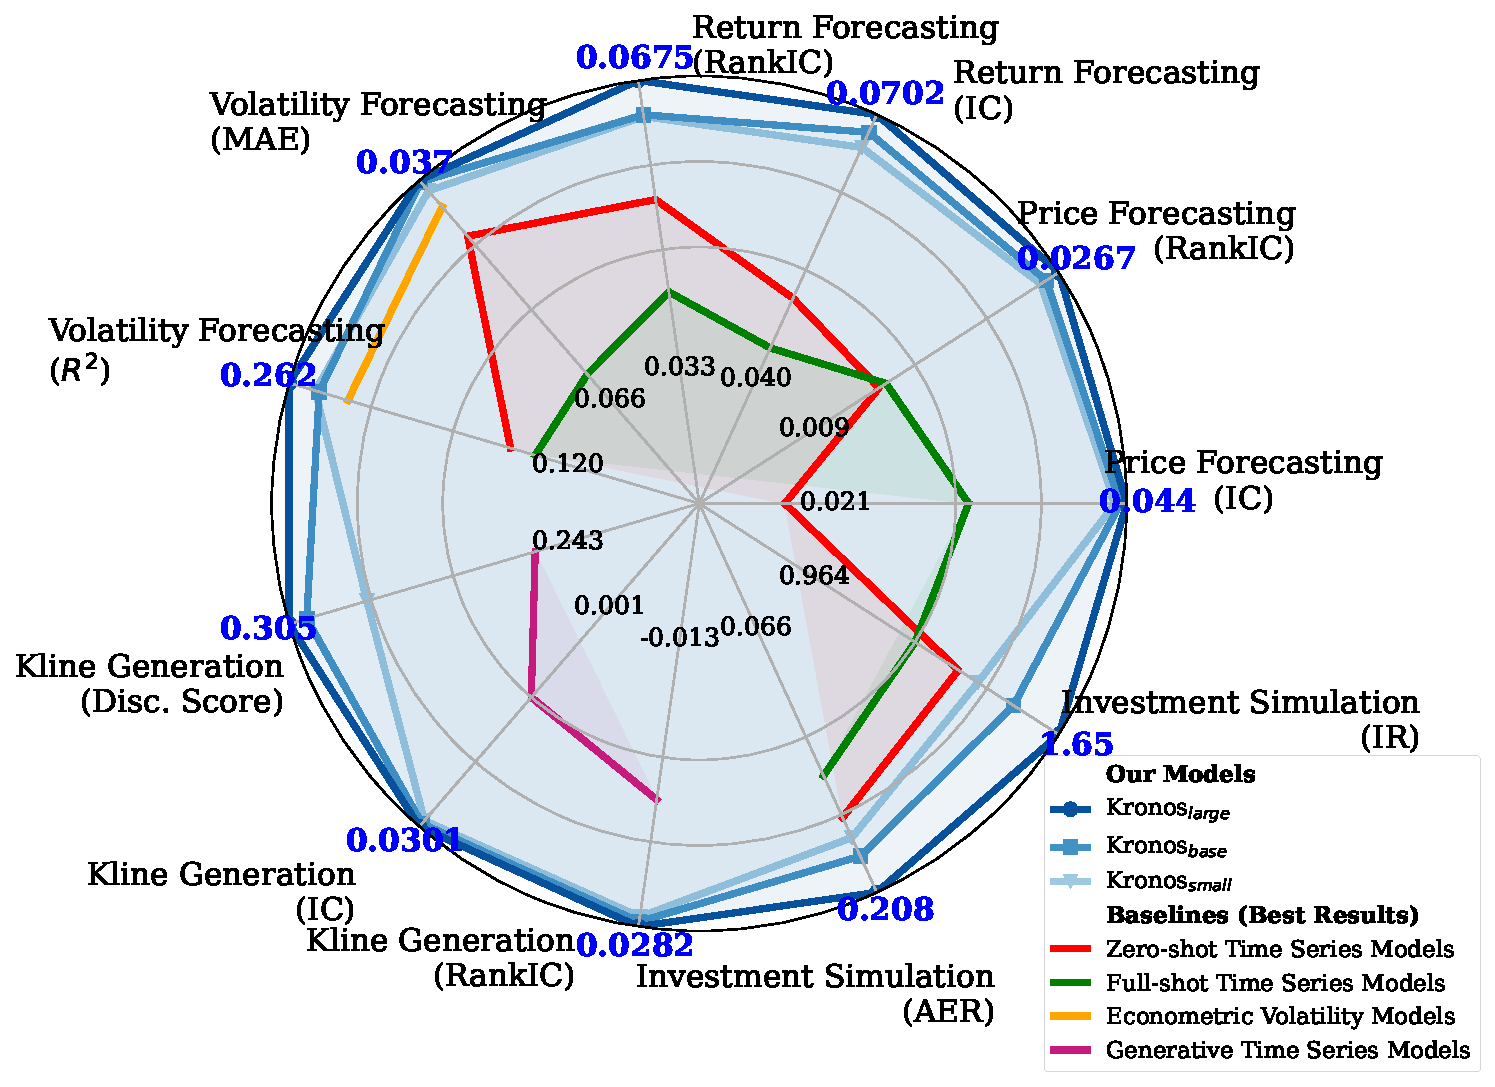
\includegraphics[width=1.0\columnwidth]{img/performance_overview.pdf}
    \caption{여러 정량 금융 과제에서 Kronos의 종합 성능. 이 차트는 우리의 Kronos 모델들(파란색 계열)을 여러 범주의 특화된 베이스라인과 비교한다.
    중심에서 더 멀리 떨어질수록 더 우수한 성능을 의미한다.
    }
    \label{fig:performance_overview}
\end{figure}


그러나 범용 TSFMs를 금융 K-line 데이터에 적용하는 것은 두 가지 주요 요인으로 인해 상당한 도전을 제기한다.
첫째, K-line 시퀀스는 낮은 신호대잡음비, 강한 비정상성, OHLCVA 속성들 사이의 복잡한 고차 의존성~\cite{zhang2025major,baidya2024addressing}과 같은 고유한 통계적 특성을 보이는데, 이는 일반적인 TSFMs의 귀납적 편향과 잘 맞지 않는 경우가 많다.
둘째, 금융 도메인은 주류 TSFM 연구에서 대체로 충분히 다루어지지 않았다; 금융 시퀀스는 대부분의 기존 TSFMs~\cite{das2024decoder,gao2024units,xiaoming2025time}의 사전학습 코퍼스에서 작은 비중만을 차지하며
, 변동성 추정, 합성 시퀀스 생성, 리스크 관리에 걸친 정량 금융에 중요한 다운스트림 과제의 범위는 대체로 해결되지 않은 채 남아 있다. 이러한 요인들은 중요한 관찰로 이어지며, 우리는 이를 본 연구에서 실증적으로 검증한다: 범용 TSFMs는 금융 과제에서 특화된 사전학습되지 않은 모델(예: iTransformer~\cite{liuitransformer})보다 성능이 낮은 경우가 많고, 더 넓은 정량 금융 지형 전반으로 일반화하는 데 실패한다.

이러한 한계를 해결하기 위해, 우리는 \textbf{금융 K-line 데이터를 위해 특별히 설계된 통합적이고 확장 가능한 사전학습 프레임워크인 Kronos}를 소개한다. Kronos는 특화된 토크나이저를 사용하여 연속적인 다변량 K-line 입력을 조밀한 토큰 시퀀스로 이산화하고, 중요한 가격--거래량 상호작용을 보존한다. 이후 45개 이상의 글로벌 시장과 7개의 시간적 세분도에서 추출한 120억 개 이상의 K-line 기록으로 구성된 방대하고 이질적인 코퍼스에서 자기회귀 사전학습을 수행한다.

우리는 다양한 정량 금융 과제 전반에 걸친 포괄적인 실험을 통해 Kronos의 효용성을 검증하며, 그 상위 수준 요약은 Figure \ref{fig:performance_overview}에 제시되어 있다. 핵심 과제인 가격 시계열 예측에서 Kronos는 새로운 state-of-the-art를 수립하며, RankIC를 선도적인 TSFM 대비 93\%, 최고 성능의 사전학습되지 않은 베이스라인 대비 87\% 향상시킨다. 또한 변동성 예측에서 9\% 더 낮은 MAE를 달성하고 합성 K-line 생성의 생성 충실도를 22\% 개선함으로써 강한 범용성을 보여준다. 이러한 결과는 우리의 접근법이 폭넓게 효과적임을 강조하고, 금융 시장의 복잡한 ``언어''를 해석하기 위한 견고한 foundation model로서 Kronos의 잠재력을 부각한다.

우리의 주요 기여는 다음과 같이 요약할 수 있다:

\begin{itemize}
    \item 우리는 계층적 표현을 학습하는 금융 K-line 데이터를 위한 새로운 모델링 프레임워크를 제안한다. 이 프레임워크는 각 다변량 K-line 기록을 구조화된 이중 구성요소(거친 및 세밀한) 토큰으로 양자화하는 특화된 토크나이저와, 이러한 서브토큰을 순차적으로 예측하는 맞춤형 자기회귀 목표를 특징으로 한다. 이 coarse-to-fine 예측 방식은 Kronos가 다중 스케일 시장 동학을 명시적으로 모델링할 수 있게 한다.

    \item 우리는 다양한 용량을 가진 Kronos 모델군에 대해 대규모 사전학습을 수행한다. 이는 45개 이상의 글로벌 거래소에서 수집한 120억 개 이상의 K-line 기록으로 구성된 방대하고 다양한 금융 코퍼스에서 수행되며, 모델들의 효과성을 뒷받침하는 견고하고 일반화 가능한 시장 표현을 학습하는 데 핵심적이다.

    \item 우리는 일련의 정량 금융 과제 전반에 대해 포괄적인 실증 평가를 수행한다. 우리의 결과는 Kronos가 가격 시계열 예측에서 새로운 state-of-the-art를 수립하며, TSFMs와 특화된 베이스라인 모두를 상당히 능가함을 보여준다. 모델의 범용성은 변동성 예측과 합성 K-line 생성을 포함한 더 넓은 범위의 정량 과제에서 보이는 강력한 성능으로 추가 입증된다.
\end{itemize}

\begin{figure*}[t!]
    \centering
    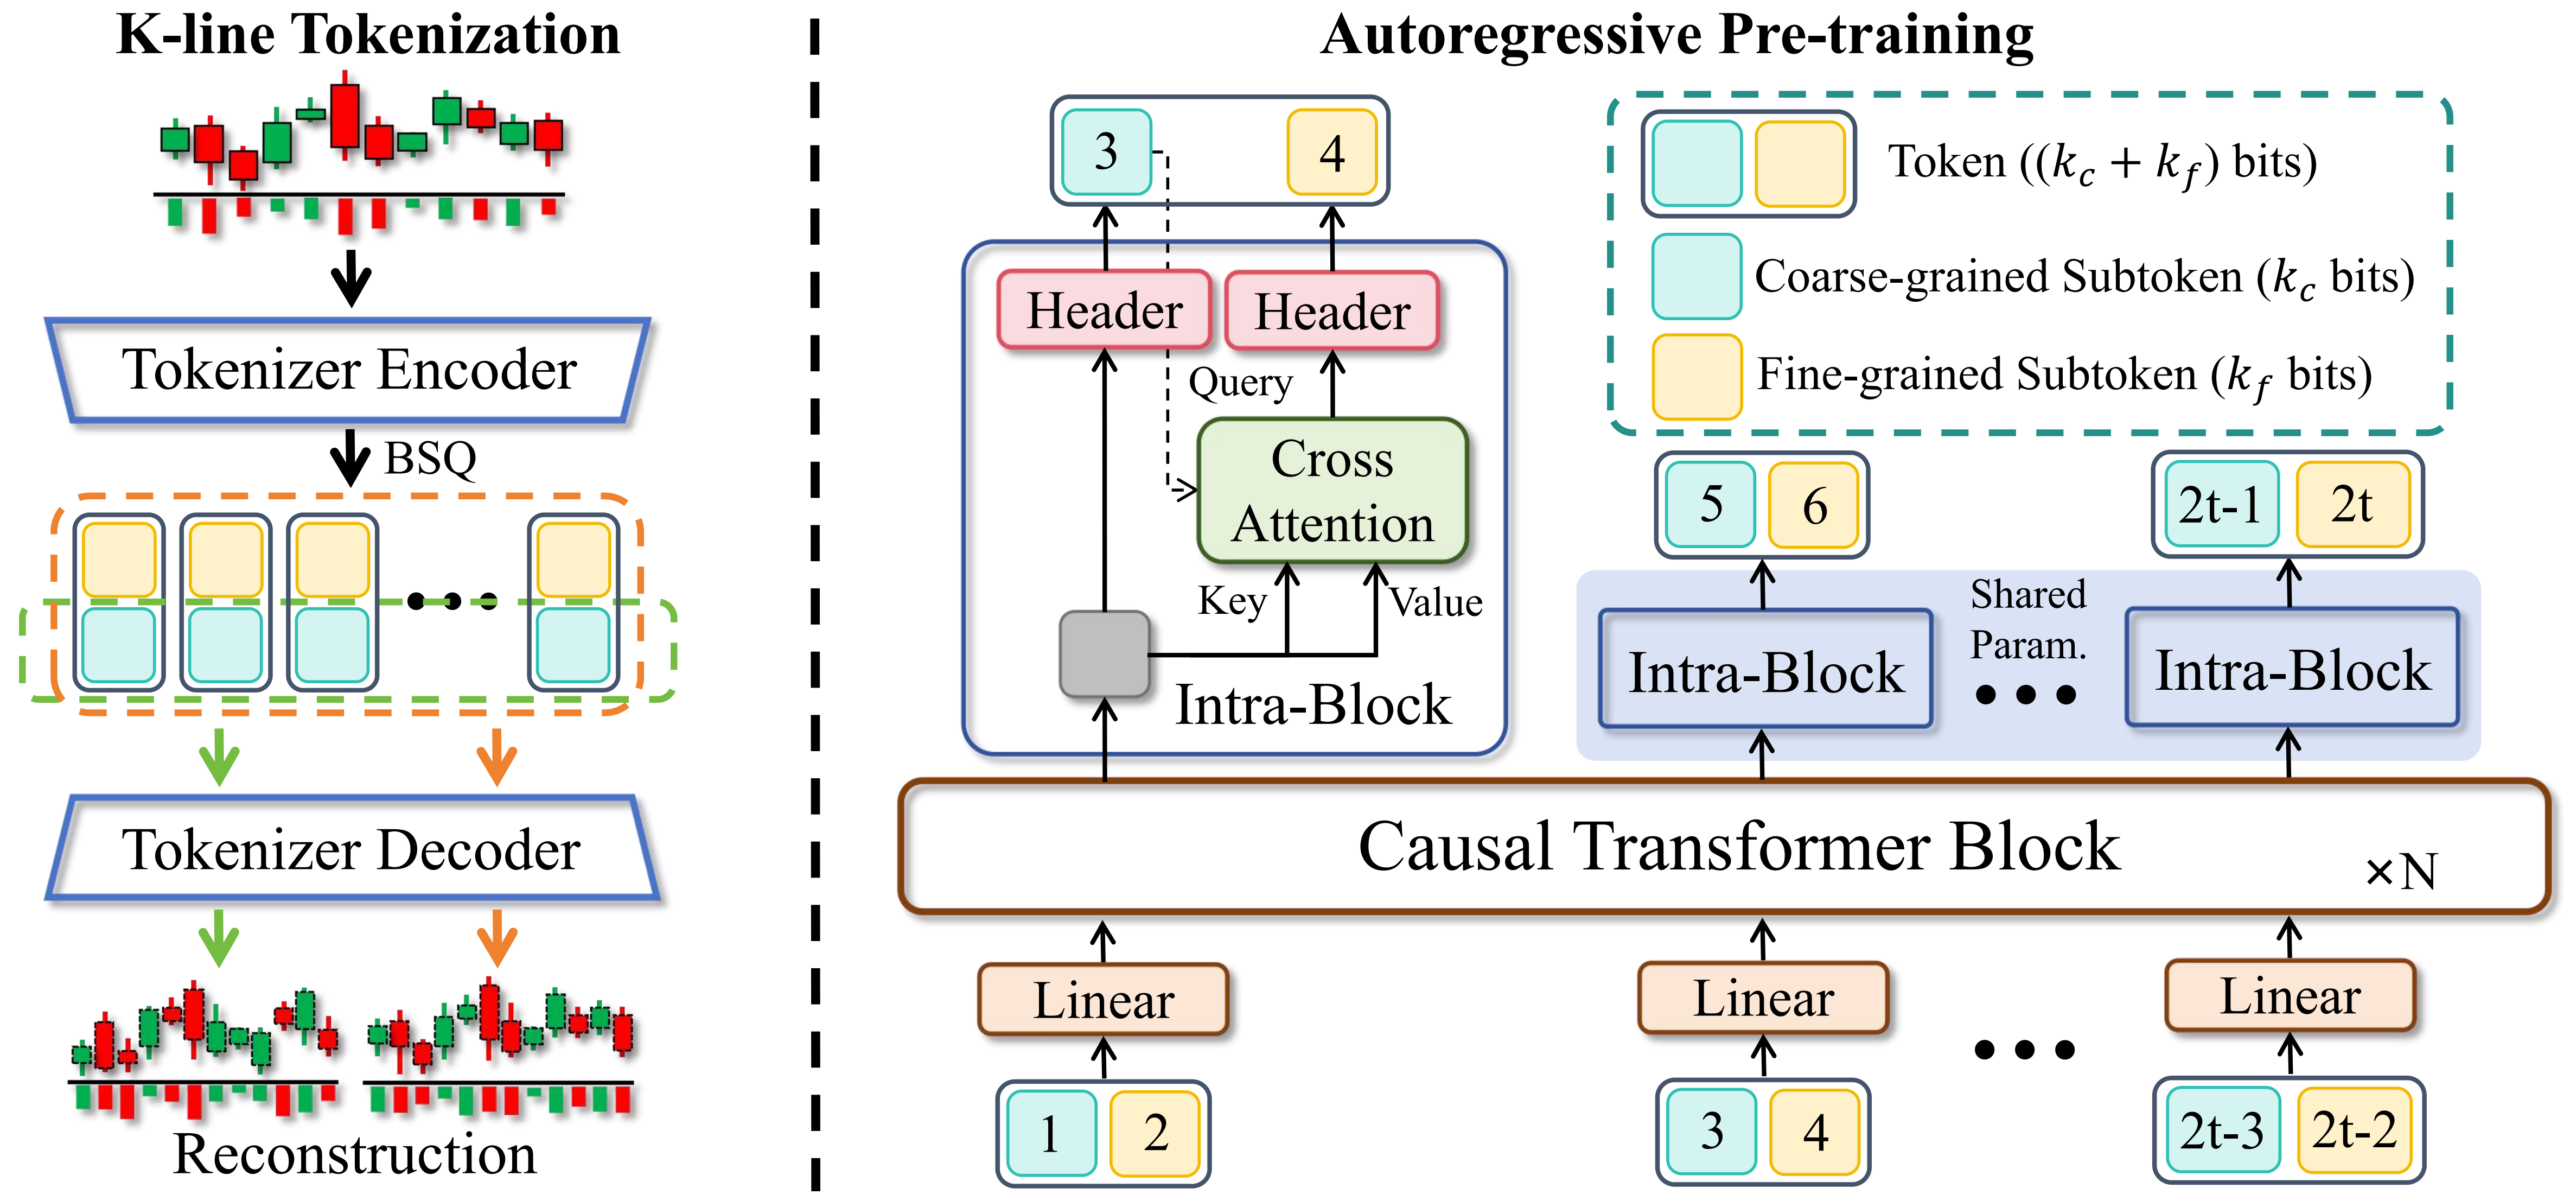
\includegraphics[width=1.0\textwidth]{img/Overview.png}
    \caption{Kronos의 2단계 프레임워크. \textbf{(1) Instance-based K-line Tokenization:} 이중 재구성 목표를 갖는 Transformer 기반 오토인코더가 연속적인 K-line 데이터를 계층적 이산 토큰의 어휘로 양자화하며, 각 토큰은 거친 서브토큰과 세밀한 서브토큰으로 구성된다. \textbf{(2) Autoregressive Pre-training:} decoder-only Transformer는 과거를 조건으로 다음 시점의 계층적 서브토큰을 순차적으로 예측함으로써 시간 동학을 모델링하도록 사전학습된다.}
    \label{fig:overview}
\end{figure*}
